\section{Results}



\begin{figure*}[!t]
	\centering
	%	\Large{Average performance on different tournament size - Gallagher's Gaussian 21-hi Peaks Function}
	\begin{subfigure}[b]{0.33\textwidth}
		\centering
		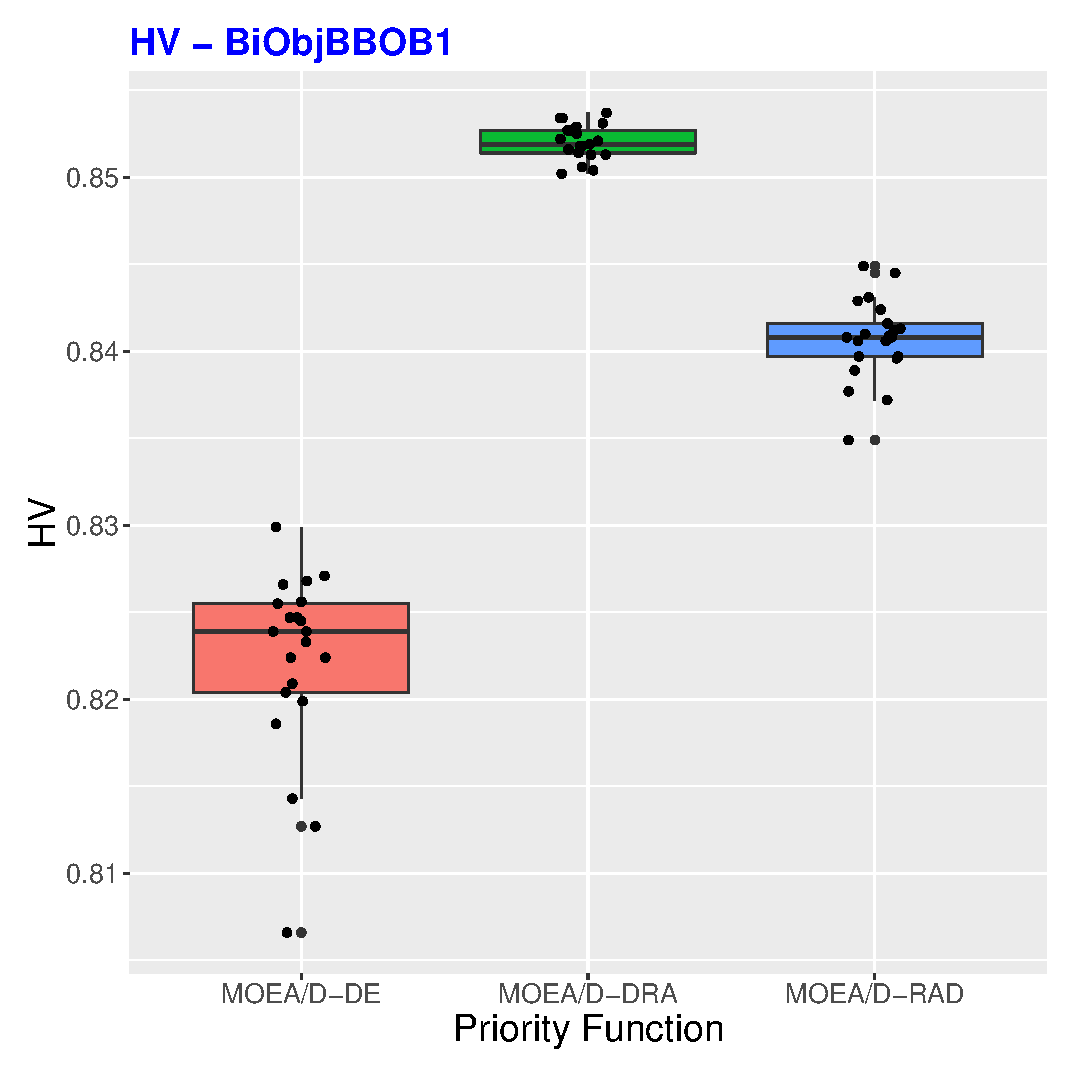
\includegraphics[width=1\textwidth, height=1\textwidth]{img/BiObjBBOB1_HV.eps}
		%	\caption{HV - UF3}
	\end{subfigure}
	\begin{subfigure}[b]{0.33\textwidth}
		\centering
		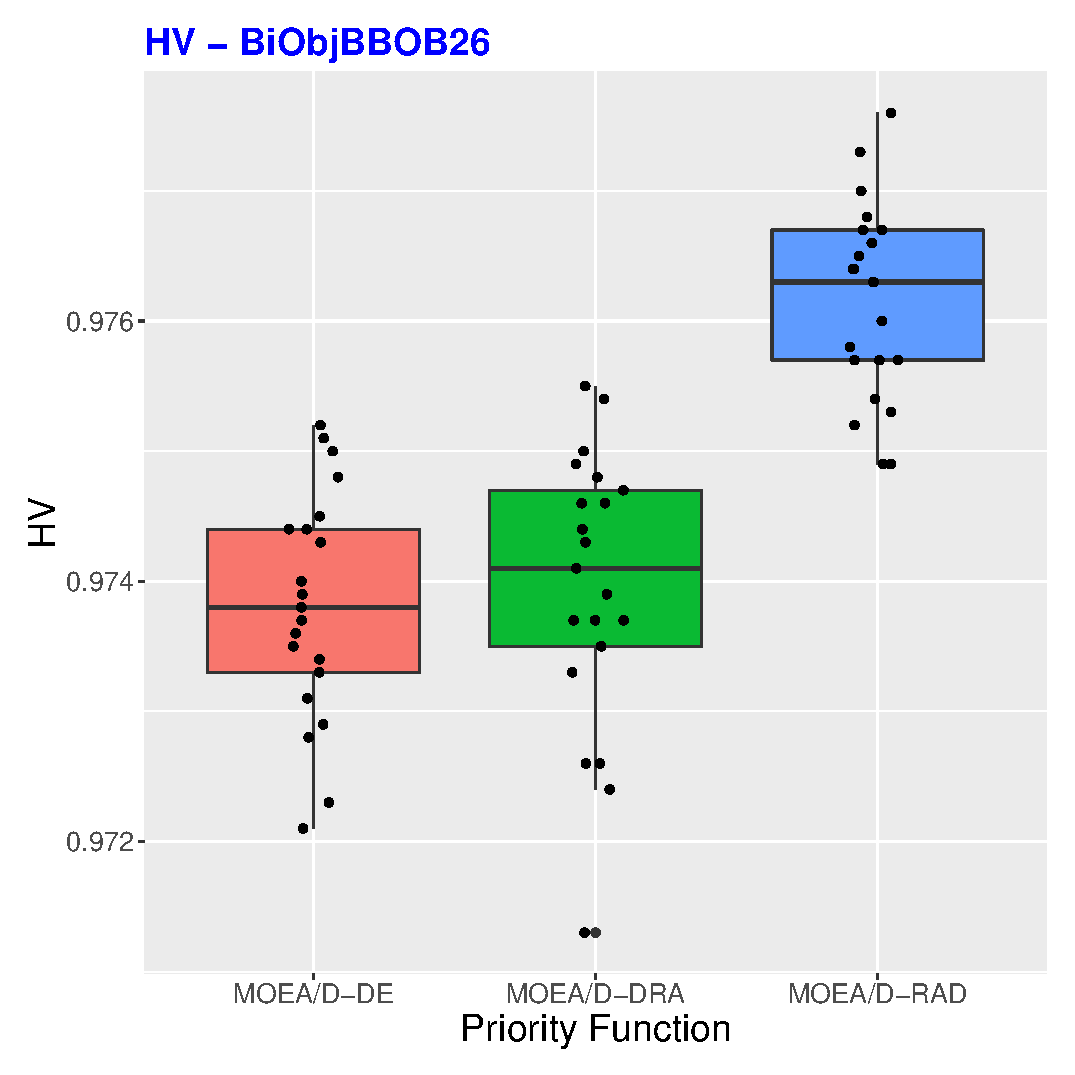
\includegraphics[width=1\textwidth, height=1\textwidth]{img/BiObjBBOB26_HV.eps}
		%	\caption{HV - UF8}
	\end{subfigure}
	\begin{subfigure}[b]{0.33\textwidth}
		\centering
		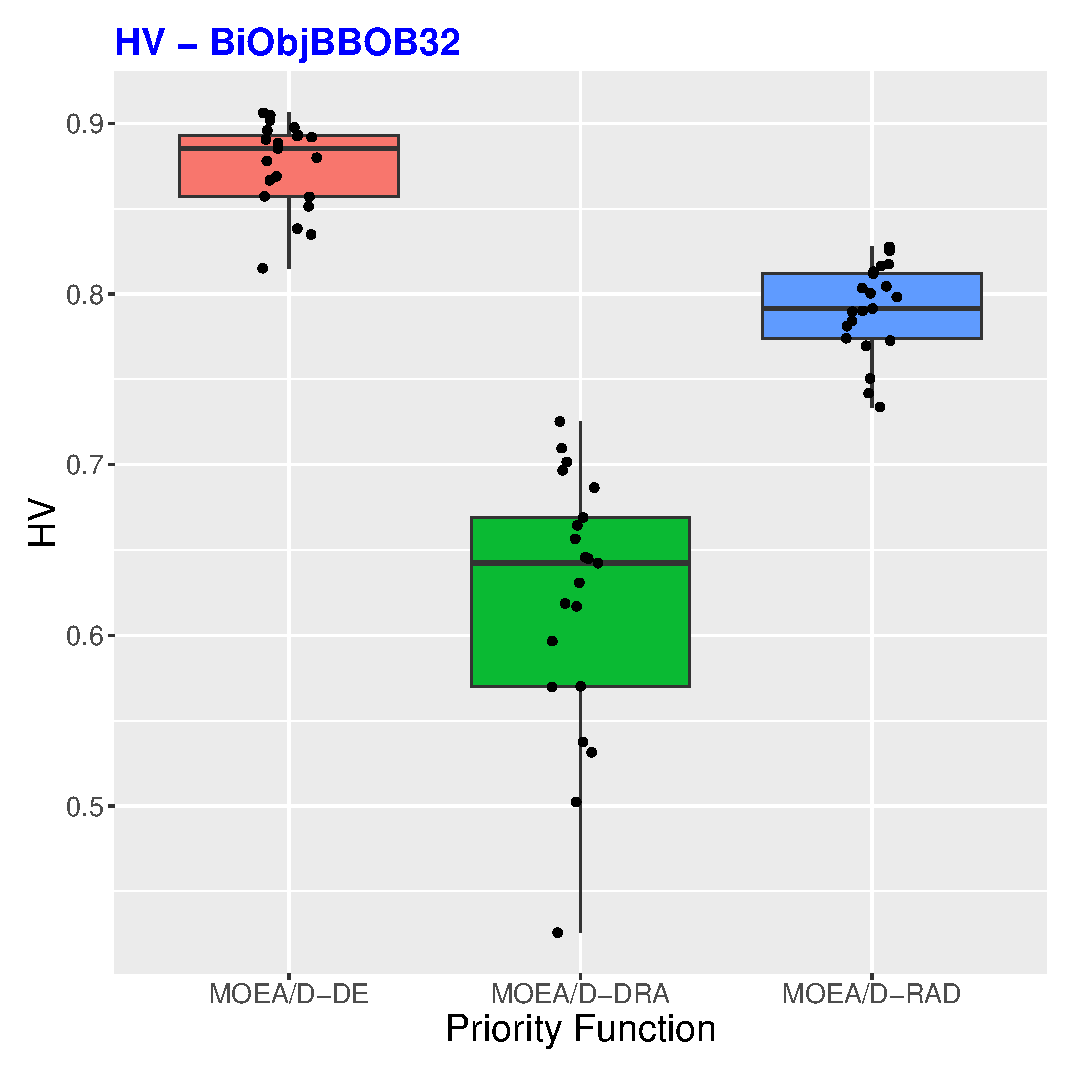
\includegraphics[width=1\textwidth, height=1\textwidth]{img/BiObjBBOB32_HV.eps}
		%	\caption{HV - DTLZ4}
	\end{subfigure}
	\caption{Box plot of HV values on  bbob-biobj-1,  bbob-biobj-26 and  bbob-biobj-32. (Higher values are better)}
	\label{HVS}
\end{figure*}

\begin{figure*}[!t]
	\centering
	%	\Large{Average performance on different tournament size - Gallagher's Gaussian 21-hi Peaks Function}
	\begin{subfigure}[b]{0.33\textwidth}
		\centering
		\includegraphics[width=1\textwidth, height=0.8\textwidth]{img/RA-DRA-26.eps}
	\end{subfigure}
	\begin{subfigure}[b]{0.33\textwidth}
		\centering
		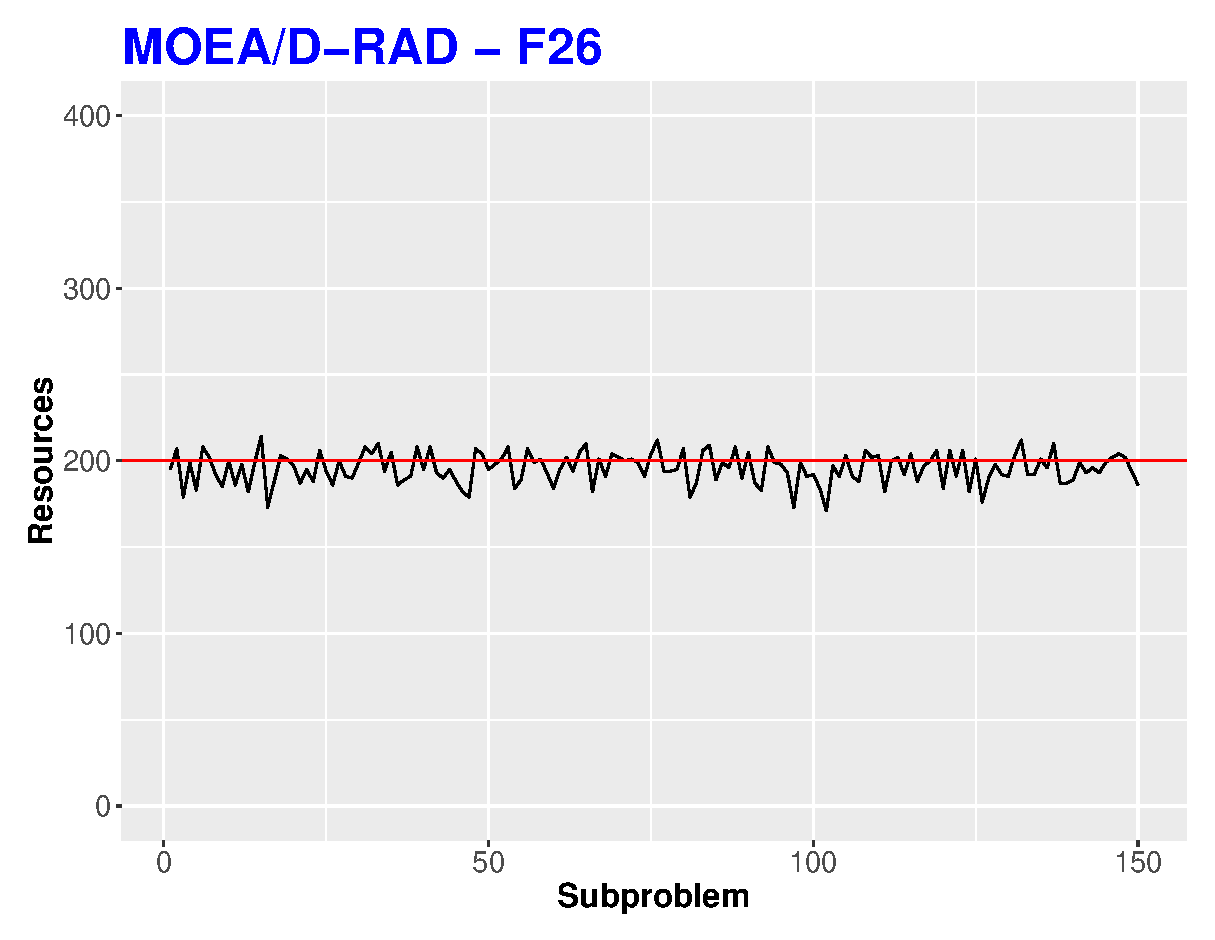
\includegraphics[width=1\textwidth, height=0.8\textwidth]{img/RA-RAD-26.eps}
	\end{subfigure}
	\caption{Resource Allocation by subproblem - The red line indicates the default amount of resource for each problem, i.e., with no priority function.}
	\label{RAs1}
\end{figure*}

\begin{figure*}[!t]
	\centering
	\begin{subfigure}[b]{0.33\textwidth}
		\centering
		\includegraphics[width=1\textwidth, height=0.8\textwidth]{img/RA-DRA-32.eps}
	\end{subfigure}
	\begin{subfigure}[b]{0.33\textwidth}
		\centering
		\includegraphics[width=1\textwidth, height=0.8\textwidth]{img/RA-RAD-32.eps}
	\end{subfigure}
	\caption{Resource Allocation by subproblem - The red line indicates the default amount of resource for each problem, i.e., with no priority function.}
	\label{RAs2}
\end{figure*}

\begin{center}

\begin{table*}[!t]
	\tabcolsep=0.33cm
	\footnotesize
	\begin{tabular}{ccccccc}
		\cline{7-7}
		\hline

		\rowcolor[gray]{.5} \multicolumn{1}{|c}{Metric} & \multicolumn{3}{|c|}{HV} &     \multicolumn{3}{c|}{Proportion of Non-dominated} \\ \hline \hline  \hline
		\multicolumn{1}{|l}{Algorithm: }  & \multicolumn{1}{|l|}{MOEA/D-DE} & \multicolumn{1}{l|}{MOEA/D-RAD} & \multicolumn{1}{l|}{MOEA/D-DRA} &  \multicolumn{1}{l|}{MOEA/D-DE} & \multicolumn{1}{l|}{MOEA/D-RAD} & \multicolumn{1}{l|}{MOEA/D-DRA}
		\\ \hline \hline
		\multicolumn{1}{|l|}{Group 1 - F1.}           & \multicolumn{1}{l}{0.8239 (0.005)} & \multicolumn{1}{l}{0.8408 (0.002) } & \multicolumn{1}{l|}{\textbf{0.8519 (0.001)}}
		& \multicolumn{1}{l}{0.460 (0.07)} & \multicolumn{1}{l}{0.910 (0.09) } & \multicolumn{1}{l|}{1.000 (0.00)} \\ \hline
		\rowcolor[gray]{.85} \multicolumn{1}{|l|}{Group 1 - F2.}              & \multicolumn{1}{l}{0.9480 (0.003)} & \multicolumn{1}{l}{\textbf{0.9572 (0.001)}} & \multicolumn{1}{l|}{0.6435 (0.043)} &		 \multicolumn{1}{l}{0.3933 (0.05)} & \multicolumn{1}{l}{0.800 (0.08) } & \multicolumn{1}{l|}{0.9933 (0.04)} \\ \hline
		\rowcolor[gray]{.85}  \multicolumn{1}{|l|}{Group 2 - F3.}           & \multicolumn{1}{l}{0.9113 (0.002)} & \multicolumn{1}{l}{\textbf{0.9211 (0.001)}} & \multicolumn{1}{l|}{0.5783  (0.043)} & \multicolumn{1}{l}{0.4800 (0.06)} & \multicolumn{1}{l}{0.9133 (0.12)} & \multicolumn{1}{l|}{0.9933 (0.04)}  \\ \hline
		\rowcolor[gray]{.85}  \multicolumn{1}{|l|}{Group 2 - F4.}              & \multicolumn{1}{l}{0.9392 (0.002)} & \multicolumn{1}{l}{\textbf{0.9477 (0.002)}} & \multicolumn{1}{l|}{0.7236 (0.018)}  & \multicolumn{1}{l}{0.4267 (0.06)} & \multicolumn{1}{l}{0.8267 (0.06)} & \multicolumn{1}{l|}{1.0000 (0.01)}  \\ \hline
		\multicolumn{1}{|l|}{Group 3 - F5.}  & \multicolumn{1}{l}{0.6722 (0.008)} & \multicolumn{1}{l}{0.6937 (0.006)} & \multicolumn{1}{l|}{\textbf{0.7024 (0.003)}}  & \multicolumn{1}{l}{0.4867 (0.07)} & \multicolumn{1}{l}{0.9067 (0.07)} & \multicolumn{1}{l|}{1.000 (0.01)}   \\ \hline
		\multicolumn{1}{|l|}{Group 3 - F6.}         & \multicolumn{1}{l}{0.8946 (0.003)} & \multicolumn{1}{l}{0.9092 (0.003)} & \multicolumn{1}{l|}{\textbf{0.9146 (0.002)}}		& \multicolumn{1}{l}{0.4533 (0.05)} & \multicolumn{1}{l}{0.8467 (0.06)} & \multicolumn{1}{l|}{1.000 (0.00)} 		 \\ \hline
		\rowcolor[gray]{.85}  \multicolumn{1}{|l|}{Group 4 - F7.}  & \multicolumn{1}{l}{0.8313 (0.008)} & \multicolumn{1}{l}{\textbf{0.8350 (0.018)}} & \multicolumn{1}{l|}{0.8173 (0.017)}  & \multicolumn{1}{l}{0.3600 (0.04)} & \multicolumn{1}{l}{0.8533 (0.09)} & \multicolumn{1}{l|}{0.9933 (0.03)}	\\ \hline
		\multicolumn{1}{|l|}{Group 4 -F8.}              & \multicolumn{1}{l}{\textbf{0.8784 (0.016)}} & \multicolumn{1}{l}{0.8159 (0.032)} & \multicolumn{1}{l|}{0.7500 (0.031)} 		& \multicolumn{1}{l}{0.3533 (0.06)} & \multicolumn{1}{l}{0.8533 (0.11)} & \multicolumn{1}{l|}{1.000 (0.02)}  \\ \hline
		\rowcolor[gray]{.85} \multicolumn{1}{|l|}{Group 5 - F9.}           & \multicolumn{1}{l}{0.9526 (0.002)} & \multicolumn{1}{l}{\textbf{0.9583 (0.081)}} & \multicolumn{1}{l|}{0.8340 (0.002)}  		& \multicolumn{1}{l}{0.4533 (0.08)} & \multicolumn{1}{l}{0.867 (0.06)} & \multicolumn{1}{l|}{1.000 (0.04)}  \\ \hline
		\rowcolor[gray]{.85} \multicolumn{1}{|l|}{Group 5 - F10.}              & \multicolumn{1}{l}{0.7780 (0.030)} & \multicolumn{1}{l}{\textbf{0.7882 (0.031)}} & \multicolumn{1}{l|}{0.7484 (0.038)}  		 & \multicolumn{1}{l}{0.5267 (0.07)} & \multicolumn{1}{l}{0.8667 (0.07)} & \multicolumn{1}{l|}{1.000 (0.00)}  \\ \hline
		\multicolumn{1}{|l|}{Group 1 - F11.}           & \multicolumn{1}{l}{0.8214 (0.003)} & \multicolumn{1}{l}{0.8315 (0.001)} & \multicolumn{1}{l|}{\textbf{0.8398 (0.000)}}  	& \multicolumn{1}{l}{0.6000 (0.06)} & \multicolumn{1}{l}{0.9200 (0.05)} & \multicolumn{1}{l|}{1.000 (0.00)}  \\ \hline
		\rowcolor[gray]{.85}  \multicolumn{1}{|l|}{Group 2 - F12.}              & \multicolumn{1}{l}{0.9945 (0.001)} & \multicolumn{1}{l}{\textbf{0.9948 (0.001)}} & \multicolumn{1}{l|}{0.9876 (0.005)}  & \multicolumn{1}{l}{0.4533 (0.08)} & \multicolumn{1}{l}{0.8933 (0.09)} & \multicolumn{1}{l|}{1.000 (0.00)}  \\ \hline
		\rowcolor[gray]{.85}  \multicolumn{1}{|l|}{Group 2 - F13.}           & \multicolumn{1}{l}{0.9890 (0.001)} & \multicolumn{1}{l}{\textbf{0.9907 (0.001)}} & \multicolumn{1}{l|}{0.9855 (0.003)}  	& \multicolumn{1}{l}{0.4200 (0.07)} & \multicolumn{1}{l}{0.8200 (0.11)} & \multicolumn{1}{l|}{1.000 (0.00)}  \\ \hline
		\rowcolor[gray]{.85}  \multicolumn{1}{|l|}{Group 3 - F14.}              & \multicolumn{1}{l}{0.8995 (0.008)} & \multicolumn{1}{l}{\textbf{0.9155 (0.009)}} & \multicolumn{1}{l|}{0.6580 (0.056)}  		& \multicolumn{1}{l}{0.48733 (0.05)} & \multicolumn{1}{l}{0.8800 (0.08)} & \multicolumn{1}{l|}{0.9933 (0.01)}  \\ \hline
		\rowcolor[gray]{.85}  \multicolumn{1}{|l|}{Group 3 - F15.}           & \multicolumn{1}{l}{0.9881 (0.002)} & \multicolumn{1}{l}{\textbf{0.9903 (0.002)}} & \multicolumn{1}{l|}{0.8981 (0.033)}  	& \multicolumn{1}{l}{0.3733 (0.06)} & \multicolumn{1}{l}{0.7333 (0.12)} & \multicolumn{1}{l|}{1.000 (0.02)}  \\ \hline
		\multicolumn{1}{|l|}{Group 4 -F16.}              & \multicolumn{1}{l}{\textbf{0.9609 (0.007)}} & \multicolumn{1}{l}{0.9449 (0.009)} & \multicolumn{1}{l|}{0.8562 (0.037)}  		& \multicolumn{1}{l}{0.3533 (0.07)} & \multicolumn{1}{l}{0.8067 (0.09)} & \multicolumn{1}{l|}{0.9867 (0.05)}  \\ \hline
		\multicolumn{1}{|l|}{Group 4 -F17.}           & \multicolumn{1}{l}{\textbf{0.9752 (0.017)}} & \multicolumn{1}{l}{0.9042 (0.022)} & \multicolumn{1}{l|}{0.7901 (0.053)}  	& \multicolumn{1}{l}{0.3000 (0.06)} & \multicolumn{1}{l}{0.7667 (0.11)} & \multicolumn{1}{l|}{0.9733 (0.13)}  \\ \hline
		\rowcolor[gray]{.85} \multicolumn{1}{|l|}{Group 5 - F18.}              & \multicolumn{1}{l}{0.9455 (0.001)} & \multicolumn{1}{l}{\textbf{0.9455 (0.001)}} & \multicolumn{1}{l|}{0.8988 (0.015)}  		& \multicolumn{1}{l}{0.4733 (0.09)} & \multicolumn{1}{l}{0.8533 (0.09)} & \multicolumn{1}{l|}{1.0000 (0.00)}  \\ \hline
		\rowcolor[gray]{.85} \multicolumn{1}{|l|}{Group 5 - F19.}           & \multicolumn{1}{l}{0.9217 (0.025)} & \multicolumn{1}{l}{\textbf{0.9441 (0.057)}} & \multicolumn{1}{l|}{0.6001 (0.182)}  	& \multicolumn{1}{l}{0.4800 (0.09)} & \multicolumn{1}{l}{0.8333 (0.11)} & \multicolumn{1}{l|}{1.000 (0.05)}  \\ \hline
		\rowcolor[gray]{.85}  \multicolumn{1}{|l|}{Group 6 - F20.}              & \multicolumn{1}{l}{0.9857 (0.001)} & \multicolumn{1}{l}{\textbf{0.9869 (0.001)}} & \multicolumn{1}{l|}{0.9868 (0.001)}  		& \multicolumn{1}{l}{0.5800 (0.09)} & \multicolumn{1}{l}{0.9333 (0.05)} & \multicolumn{1}{l|}{1.0000 (0.00)}  \\ \hline
		\multicolumn{1}{|l|}{Group 6 - F21.}           & \multicolumn{1}{l}{0.9719 (0.001)} & \multicolumn{1}{l}{0.9756 (0.001)} & \multicolumn{1}{l|}{\textbf{0.9766 (0.001)}}  	& \multicolumn{1}{l}{0.4933 (0.07)} & \multicolumn{1}{l}{0.9000 (0.09)} & \multicolumn{1}{l|}{1.000 (0.00)}  \\ \hline
		\rowcolor[gray]{.85}  \multicolumn{1}{|l|}{Group 7 - F22.}              & \multicolumn{1}{l}{0.8035 (0.006)} & \multicolumn{1}{l}{\textbf{0.8177 (0.005)}} & \multicolumn{1}{l|}{0.6182 (0.031)}  		& \multicolumn{1}{l}{0.5067 (0.08)} & \multicolumn{1}{l}{0.8800 (0.06)} & \multicolumn{1}{l|}{1.0000 (0.02)}  \\ \hline
		\rowcolor[gray]{.85}  \multicolumn{1}{|l|}{Group 7 - F23.}           & \multicolumn{1}{l}{0.9677 (0.001)} & \multicolumn{1}{l}{\textbf{0.9714 (0.001)}} & \multicolumn{1}{l|}{0.7871 (0.027)}  	& \multicolumn{1}{l}{0.4933 (0.05)} & \multicolumn{1}{l}{0.8800 (0.08)} & \multicolumn{1}{l|}{0.9933 (0.03)}  \\ \hline
		\multicolumn{1}{|l|}{Group 8 - F24.}              & \multicolumn{1}{l}{\textbf{0.9674 (0.009)}} & \multicolumn{1}{l}{0.9408 (0.013)} & \multicolumn{1}{l|}{0.8609 (0.031)}  		& \multicolumn{1}{l}{0.3933 (0.06)} & \multicolumn{1}{l}{0.7800 (0.11)} & \multicolumn{1}{l|}{0.9800 (0.12)}  \\ \hline
		\multicolumn{1}{|l|}{Group 8 - F25.}           & \multicolumn{1}{l}{\textbf{0.9699 (0.009)}} & \multicolumn{1}{l}{0.9349 (0.012)} & \multicolumn{1}{l|}{0.8647 (0.045)} & \multicolumn{1}{l}{0.3200 (0.05)} & \multicolumn{1}{l}{0.7600 (0.11)} & \multicolumn{1}{l|}{0.9533 (0.13)}  \\ \hline
		\rowcolor[gray]{.85}  \rowcolor[gray]{.85}  \multicolumn{1}{|l|}{Group 9 - F26.}              & \multicolumn{1}{l}{0.9738 (0.001)} & \multicolumn{1}{l}{\textbf{0.9763 (0.001)}} & \multicolumn{1}{l|}{0.9741 (0.001)}  		& \multicolumn{1}{l}{0.5600 (0.09)} & \multicolumn{1}{l}{0.9467 (0.05)} & \multicolumn{1}{l|}{1.0000 (0.00)}  \\ \hline
		\rowcolor[gray]{.85}  \multicolumn{1}{|l|}{Group 9 - F27.}           & \multicolumn{1}{l}{0.9437 (0.042)} & \multicolumn{1}{l}{\textbf{0.9480 (0.044)}} & \multicolumn{1}{l|}{0.6161 (0.172)} & \multicolumn{1}{l}{0.5467 (0.08)} & \multicolumn{1}{l}{0.8933 (0.06)} & \multicolumn{1}{l|}{0.9867 (0.07)}  \\ \hline
		\multicolumn{1}{|l|}{Group 6 - F28.}              & \multicolumn{1}{l}{0.9808 (0.001)} & \multicolumn{1}{l}{0.9836 (0.001)} & \multicolumn{1}{l|}{\textbf{0.9866 (0.001)}}  		& \multicolumn{1}{l}{0.4067 (0.06)} & \multicolumn{1}{l}{0.8333 (0.09)} & \multicolumn{1}{l|}{1.000 (0.00)}  \\ \hline
		\rowcolor[gray]{.85}  \multicolumn{1}{|l|}{Group 7 - F29.}           & \multicolumn{1}{l}{0.7314 (0.016)} & \multicolumn{1}{l}{\textbf{0.8589 (0.008)}} & \multicolumn{1}{l|}{0.8403 (0.009)} & \multicolumn{1}{l}{0.4600 (0.08)} & \multicolumn{1}{l}{0.8467 (0.07)} & \multicolumn{1}{l|}{1.000 (0.00)}  \\ \hline
		\rowcolor[gray]{.85}  \multicolumn{1}{|l|}{Group 7 - F30.}              & \multicolumn{1}{l}{0.9687 (0.002)} & \multicolumn{1}{l}{\textbf{0.9738 (0.002)}} & \multicolumn{1}{l|}{0.8009 (0.025}  		& \multicolumn{1}{l}{0.4600 (0.06)} & \multicolumn{1}{l}{0.8000 (0.10)} & \multicolumn{1}{l|}{0.9933 (0.03)}  \\ \hline
		\multicolumn{1}{|l|}{Group 8 - F31.}           & \multicolumn{1}{l}{\textbf{0.9255 (0.036)}} & \multicolumn{1}{l}{0.8529 (0.036)} & \multicolumn{1}{l|}{0.7477 (0.045)}		& \multicolumn{1}{l}{0.3400 (0.07)} & \multicolumn{1}{l}{0.8000 (0.08)} & \multicolumn{1}{l|}{0.9733 (0.13)}  \\ \hline
		\multicolumn{1}{|l|}{Group 8 - F32.}              & \multicolumn{1}{l}{\textbf{0.8852 (0.025)}} & \multicolumn{1}{l}{0.7915 (0.026)} & \multicolumn{1}{l|}{0.6423 (0.076)}  		& \multicolumn{1}{l}{0.3400 (0.06)} & \multicolumn{1}{l}{0.7933 (0.07)} & \multicolumn{1}{l|}{0.9733 (0.12)}  \\ \hline
		\multicolumn{1}{|l|}{Group 9 - F33.}  & \multicolumn{1}{l}{0.9849 (0.001)} & \multicolumn{1}{l}{0.9867 (0.000)} & \multicolumn{1}{l|}{\textbf{0.9885 (0.031)}}  		& \multicolumn{1}{l}{0.4400 (0.05)} & \multicolumn{1}{l}{0.7867 (0.08)} & \multicolumn{1}{l|}{1.0000 (0.00)} \\ \hline
		\rowcolor[gray]{.85}  \multicolumn{1}{|l|}{Group 9 - F34.}              & \multicolumn{1}{l}{0.8744 (0.038)} & \multicolumn{1}{l}{\textbf{0.8776 (0.031)}} & \multicolumn{1}{l|}{0.6388 (0.182)}  		& \multicolumn{1}{l}{0.5000 (0.11)} & \multicolumn{1}{l}{0.8400 (0.10)} & \multicolumn{1}{l|}{1.0000 (0.01)}  \\ \hline
		\multicolumn{1}{|l|}{Group 10 - F35.}  & \multicolumn{1}{l}{0.5550 (0.003} & \multicolumn{1}{l}{0.5831 (0.004)} & \multicolumn{1}{l|}{\textbf{0.5956 (0.003)}}  		& \multicolumn{1}{l}{0.5067 (0.07)} & \multicolumn{1}{l}{0.9000 (0.07)} & \multicolumn{1}{l|}{01.000 (0.00)} \\ \hline
		\rowcolor[gray]{.85}  \rowcolor[gray]{.85}  \multicolumn{1}{|l|}{Group 10 - F36.}              & \multicolumn{1}{l}{0.7872 (0.006)} & \multicolumn{1}{l}{\textbf{0.7983 (0.006)}} & \multicolumn{1}{l|}{0.7872 (0.006)}  		& \multicolumn{1}{l}{0.4733 (0.08)} & \multicolumn{1}{l}{0.8733 (0.09)} & \multicolumn{1}{l|}{0.9933 (0.01)}  \\ \hline
		\multicolumn{1}{|l|}{Group 11 - F37.}  & \multicolumn{1}{l}{0.7367 (0.009)} & \multicolumn{1}{l}{0.7425 (0.010)} & \multicolumn{1}{l|}{\textbf{0.7479 (0.013)}}  		& \multicolumn{1}{l}{0.4000 (0.05)} & \multicolumn{1}{l}{0.8667 (0.08)} & \multicolumn{1}{l|}{1.000 (0.01)} \\ \hline
		\multicolumn{1}{|l|}{Group 11 - F38.}              & \multicolumn{1}{l}{\textbf{0.8619 (0.010)}} & \multicolumn{1}{l}{0.8550 (0.011)} & \multicolumn{1}{l|}{0.8461 (0.019)}  		& \multicolumn{1}{l}{0.3133 (0.05)} & \multicolumn{1}{l}{0.8667 (0.07)} & \multicolumn{1}{l|}{0.9867 (0.04)}  \\ \hline
		\rowcolor[gray]{.85}  \multicolumn{1}{|l|}{Group 12 - F39.}  & \multicolumn{1}{l}{0.8128 (0.005)} & \multicolumn{1}{l}{\textbf{0.8285 (0.004)}} & \multicolumn{1}{l|}{0.7280 (0.015)}  		& \multicolumn{1}{l}{0.5067 (0.08)} & \multicolumn{1}{l}{0.9000 (0.07)} & \multicolumn{1}{l|}{1.0000 (0.00)} \\
		\hline
		\rowcolor[gray]{.85}  \multicolumn{1}{|l|}{Group 12 - F40.}              & \multicolumn{1}{l}{0.4736 (0.047)} & \multicolumn{1}{l}{\textbf{0.5116 (0.048)}} & \multicolumn{1}{l|}{0.3954 (0.042)}  		& \multicolumn{1}{l}{0.6333 (0.08)} & \multicolumn{1}{l}{0.9467 (0.03)} & \multicolumn{1}{l|}{1.0000 (0.01)}  \\ \hline
		\multicolumn{1}{|l|}{Group 10 - F41.}  & \multicolumn{1}{l}{0.9281 (0.0.003)} & \multicolumn{1}{l}{0.9368 (0.004)} & \multicolumn{1}{l|}{\textbf{0.9480 (0.003)}}  		& \multicolumn{1}{l}{0.4133 (0.06)} & \multicolumn{1}{l}{0.8267 (0.10)} & \multicolumn{1}{l|}{1.0000 (0.00} \\ \hline
		\multicolumn{1}{|l|}{Group 11 - F42.}              & \multicolumn{1}{l}{\textbf{0.9379 (0.010)}} & \multicolumn{1}{l}{0.9034 (0.021)} & \multicolumn{1}{l|}{0.8975 (0.021)}  		& \multicolumn{1}{l}{0.3667 (0.06)} & \multicolumn{1}{l}{0.8467 (0.08)} & \multicolumn{1}{l|}{0.9933 (0.03)}  \\ \hline
		\multicolumn{1}{|l|}{Group 11 - F43.}  & \multicolumn{1}{l}{\textbf{0.8744 (0.026)}} & \multicolumn{1}{l}{0.7937 (0.031)} & \multicolumn{1}{l|}{0.7410 (0.060)}  		& \multicolumn{1}{l}{0.3733 (0.07)} & \multicolumn{1}{l}{0.7800 (0.10)} & \multicolumn{1}{l|}{0.9533 (0.15} \\ \hline
		\rowcolor[gray]{.85}  \multicolumn{1}{|l|}{Group 12 - F44.}              & \multicolumn{1}{l}{0.9687 (0.003)} & \multicolumn{1}{l}{\textbf{0.9761 (0.002}} & \multicolumn{1}{l|}{0.9032 (0.011)}  		& \multicolumn{1}{l}{0.4067 (0.06)} & \multicolumn{1}{l}{0.8200 (0.08)} & \multicolumn{1}{l|}{0.9867 (0.04)} \\ \hline
		\multicolumn{1}{|l|}{Group 12 - F45.}  & \multicolumn{1}{l}{0.8091 (0.043)} & \multicolumn{1}{l}{0.8223 (0.052)} & \multicolumn{1}{l|}{\textbf{0.8557 (0.063)}}  		& \multicolumn{1}{l}{0.5200 (0.07)} & \multicolumn{1}{l}{0.8867 (0.05)} & \multicolumn{1}{l|}{1.0000 (0.01} \\ \hline
		\multicolumn{1}{|l|}{Group 13 - F46.}              & \multicolumn{1}{l}{\textbf{0.8817 (0.012)}} & \multicolumn{1}{l}{0.8428 (0.023} & \multicolumn{1}{l|}{0.8378 (0.027)}  		& \multicolumn{1}{l}{0.2933 (0.06)} & \multicolumn{1}{l}{0.8467 (0.09)} & \multicolumn{1}{l|}{1.000 (0.03)}  \\ \hline
		\multicolumn{1}{|l|}{Group 13 - F47.}  & \multicolumn{1}{l}{\textbf{0.8208 (0.031)}} & \multicolumn{1}{l}{0.6803 (0.043)} & \multicolumn{1}{l|}{0.5553 (0.071)}  		& \multicolumn{1}{l}{0.4000 (0.08)} & \multicolumn{1}{l}{0.8667 (0.08)} & \multicolumn{1}{l|}{0.9933 (0.04} \\ \hline
		\multicolumn{1}{|l|}{Group 14 - F48.} & \multicolumn{1}{l}{\textbf{0.9520 (0.0018)}} & \multicolumn{1}{l}{0.8673 (0.033)} & \multicolumn{1}{l|}{0.7799 (0.044)} & \multicolumn{1}{l}{0.3400 (0.07)} & \multicolumn{1}{l}{0.7067 (0.13)} & \multicolumn{1}{l|}{0.9733 (0.17)}  \\ \hline
		\multicolumn{1}{|l|}{Group 14 - F49.}  & \multicolumn{1}{l}{\textbf{0.8967 (0.051)}} & \multicolumn{1}{l}{0.8730 (0.059)} & \multicolumn{1}{l|}{0.8579 (0.068)}  		& \multicolumn{1}{l}{0.4533 (0.07)} & \multicolumn{1}{l}{0.8533 (0.07)} & \multicolumn{1}{l|}{1.000 (0.03} \\ \hline
		\multicolumn{1}{|l|}{Group 13 - F50.}              & \multicolumn{1}{l}{\textbf{0.8794 (0.036)}} & \multicolumn{1}{l}{0.7626 (0.038)} & \multicolumn{1}{l|}{0.7402 (0.031)}  		& \multicolumn{1}{l}{0.3667 (0.07)} & \multicolumn{1}{l}{0.8600 (0.07)} & \multicolumn{1}{l|}{1.000 (0.01)}  \\ \hline% \hline \hline
		\multicolumn{1}{|l|}{Group 14 - F51.}  & \multicolumn{1}{l}{\textbf{0.9801 (0.008)}} & \multicolumn{1}{l}{0.9535 (0.009)} & \multicolumn{1}{l|}{0.9218 (0.017)}  		& \multicolumn{1}{l}{0.3467 (0.06)} & \multicolumn{1}{l}{0.8000 (0.11)} & \multicolumn{1}{l|}{0.9667 (0.20} \\ \hline
		\multicolumn{1}{|l|}{Group 14 - F52.}              & \multicolumn{1}{l}{\textbf{0.8839 (0.060)}} & \multicolumn{1}{l}{0.8652 (0.069)} & \multicolumn{1}{l|}{0.8414 (0.074)}  		& \multicolumn{1}{l}{0.4067 (0.07)} & \multicolumn{1}{l}{0.8533 (0.10)} & \multicolumn{1}{l|}{1.0000 (0.109)}  \\ \hline % \hline \hline
		\multicolumn{1}{|l|}{Group 15 - F53.}  & \multicolumn{1}{l}{0.9927 (0.000)} & \multicolumn{1}{l}{0.9929 (0.000)} & \multicolumn{1}{l|}{\textbf{0.9930 (0.00)}}  		& \multicolumn{1}{l}{0.5267 (0.05)} & \multicolumn{1}{l}{0.8600 (0.06)} & \multicolumn{1}{l|}{1.0000 (0.00} \\ \hline
		\multicolumn{1}{|l|}{Group 15 - F54.}              & \multicolumn{1}{l}{\textbf{0.8950 (0.045)}} & \multicolumn{1}{l}{0.8717 (0.057)} & \multicolumn{1}{l|}{0.7629 (0.135)}  		& \multicolumn{1}{l}{0.5267 (0.08)} & \multicolumn{1}{l}{0.9000 (0.07)} & \multicolumn{1}{l|}{1.000 (0.02)}  \\ \hline
		\multicolumn{1}{|l|}{Group 15 - F55.}  & \multicolumn{1}{l}{\textbf{0.3855 (0.070)}} & \multicolumn{1}{l}{0.3769 (0.084)} & \multicolumn{1}{l|}{0.3709 (0.111)}  		& \multicolumn{1}{l}{0.8867 (0.07)} & \multicolumn{1}{l}{0.9733 (0.02)} & \multicolumn{1}{l|}{1.000 (0.00} \\ \hline \hline \hline
	\end{tabular}
	\caption{On the left side, HV medians and standard deviations, in parenthesis for every function/priority function. The best values found by a priority function are in bold. On the right side, mean of the percentage of the median values and mean of the median values of the standard deviation (in parenthesis) of non-dominated solutions for every function/priority function.}
	\label{stats}
\end{table*}
\end{center}

\begin{table}[!t]
	\begin{tabular}{lll}
		\hline
		\rowcolor[gray]{.7} \multicolumn{1}{|l|}{\textbf{HV}}  & \multicolumn{1}{|l|}{MOEA/D-DRA} & \multicolumn{1}{l|}{MOEA/D-RAD} \\ \hline \hline \hline
		MOEA/D-RAD                      &  3.1e-08                      & -                                      \\
		\rowcolor[gray]{.95} MOEA/D-DE                      &  3.1e-08                   &  3.1e-08                 \\
	\end{tabular}
	\caption{Statistical Analysis of the HV results based on the Pairwise Wilcoxon Rank Sum Test. It shows that exists significant difference between MOEA/D-RAD, MOEA/D-DRA and MOEA/D-DE.}
	\label{statistics}
\end{table}

\ref{HVS} shows the boxplots of the Hypervolumes obtained by the three methods
on functions F26, F1 and F32 of BiBBOB. F26 is an example of a moderate and
weakly structured function (group 9), where MOEA/D-RAD performed best. F1  is a
separable and separable function (group 1), where MOEA/D-DRA performed best, and
F32 is a moderate and multi-modal function (group 8), where MOEA/D-DE performed
best. These figures are representative examples of their respective groups.

\ref{stats} gives us a general view of these results over all functions and
function groups. In general, MOEA/D-RAD performed better than the other methods
(or second best) in terms of hypervolume. This ranking is reinforced by a
Pairwise Wilcoxon Rank Test over the entire experiment~(\ref{statistics}).

However, a post-hoc analysis of these results focusing on the function groups
suggests some interesting properties of the three methods. We observe that
MOEA/D-RAD was specially successful for function gropus that included
moderate-conditioned or weakly-structured functions (groups 2,5,6,7,8,9,12 and
15, shaded in \ref{stats}), and performed slighly worse for groups including
multi-modal functions (groups 4,8,11,13 and 14). In particular, we find it  very
interesting that MOEA/D-DE without priority performed better in the multi-modal
groups. This post-hoc analysis suggests a follow up experiment to confirm this
observations.

\subsection{Proportion of Non-dominated Solutions}
%
%
%
Another difference that we see among the algorithms  is the proportion of non dominated solutions. The results on the~\ref{stats} indicate that MOEA/D-DRA leads to the highest rate of non-dominated solutions in the final solution set, followed by MOEA/D-RAD. In general, both substantially improve this proportion over the results of MOEA/D-DE.  It seems that there is no relation in hypervolume performance and the proportion of non-dominated solutions.


\subsection{Resource Allocation}


~\ref{RAs1} and ~\ref{RAs2} illustrate the amount resource allocated by MOEA/D-DRA and MOEA/D-RAD to every subproblem on bbob-biobj-26 and bbob-biobj-32 problems. We show images from these functions due to space limitations. We exclude the visuals from MOEA/D-DE since it give the same amount of resource to every problem (200).

It is clear from the Figures that MOEA/D-RAD and MOEA/D-DRA influence differently the Resource Allocation. It is also important to highlight that, during the execution of the algorithm, the Resource Allocation done by MOEA/D-RAD to each subproblem is similar and not very far from 200, the default amount as well as the Resource Allocation done by MOEA/D-DE. The Resource Allocation done by MOEA/D-DRA depends on the problem indicating a more adaptive behavior.
